%Usage: 
%  on the command line
%       R CMD Sweave sweaveTemplate.Rnw = Sweave sweaveTemplate
%       pdflatex sweaveTemplate
%
%  within R
%       Sweave("sweaveTemplate.tex")
%       library(tools)
%       texi2dvi("sweaveTempate.tex",pdf=TRUE)
%
% To get .R file of all the code chunks in the document:
%  on the command line
%       R CMD Stangle sweaveTemplate.Rnw = Stangle sweaveTemplate
%
%  within R
%       Stangle("sweaveTemplate.tex")
%################################################################################
\documentclass[12pt]{article}

%% set the document margins below
% The following parameters seem to provide a reasonable page setup.
% produces 1in margins, with any header or footer pushed into the margin area
%  72pt = 1in
\voffset -57pt 
\hoffset -31pt
\textwidth 468pt % 6.5in
\textheight 648pt  % 9in

%% Load any other latex packages needed
\usepackage{natbib} % bibliography style
\usepackage{graphics} % pdf bases graphics
\usepackage{amsmath} % math fonts
\usepackage{indentfirst} % intents the first paragraph of a new section
\usepackage{hyperref} % allow for hyperlinks
%% hyperref usage in text: \href{URL}{text}
\usepackage[utf8]{inputenc} % don't worry about it

%%% Declare any new math operators you may have, see section X for example usage
\DeclareMathOperator{\var}{var}
\DeclareMathOperator{\cov}{cov}

%%%%% Officially Begin the Sweave document
\usepackage{Sweave}
\begin{document}

%%% Set up any R options you might have and a good place to load base R libraries

\title{Title of the Project\\Sweave Template\\\small{course section 
(ie microarray analysis)}}  % the \\ generates a line break
\author{Matt Settles}
% date will automatically be generated
\maketitle % now actually make the title

%%###############################################################################
% Each analysis report will include the following sections and subsections
%   +Summary
%   +A brief discustion of the project/data background - overview
%     -project goals/questions
%     -description of the data
%   +Quality Assurance section
%     -any data removed based on quality
%   +Analysis Sections
%     -use a subsection for each for the major sub-parts of the analysis
%     note: make sure that both you and the reader can find and even repeat your
%        analysis based on your description.
%   +Discussion of the results and conclusions of this analysis based on
%        the above.
%     note: not to include biological interpretation
%   +If using public data which has been published, briefly compare your analysis
%        results to theirs
%   +Bibliography
%%##############################################################################
\section*{Summary}
% should not span onto page 2, keep to the first page
Single paragraph summary of the project report. Should summarize all major
sections of the report.

\newpage  % creates a page break

\tableofcontents % generates the table of contents

\section{Overview}
Provide a brief description of the project that gave rise to the data being
analyzed. Provide enough information to give the reader a general feel for 
why the work was being performed and expectations

\subsection{Analysis Objectives}
Describe the analysis objectives to the reader. The objectives will determine
what data analysis techniques are going to be performed. You can use a list here
if you like:
\begin{enumerate} % can use itemize for bullets
  \item List Item 1
  \item List Item 2
  \item List Item 3
\end{enumerate}

\subsection{Data Description}

\section{Data Quality Assurance}

\subsection{Samples removed from further analysis}

\section{Data Analysis}

The following subsections are example sub-parts of microarray analysis

\subsection{Preprocessing}
\subsection{Filtering}
\subsection{Statistical Analysis}

\section{Results}

\subsection{Comparison to Previous Analysis}

%%% Bibliography

This is an example of using the \verb@mcmc@ package in R.  The problem comes
from a take-home question on a (take-home) PhD qualifying exam
(School of Statistics, University of Minnesota).

Simulated data for the problem are in the dataset \verb@logit@.
There are five variables in the data set, the response \verb@y@
and four predictors, \verb@x1@, \verb@x2@, \verb@x3@, and \verb@x4@.

A frequentist analysis for the problem is done by the following R statements
\begin{Schunk}
\begin{Sinput}
> library(mcmc)
> data(logit)
> out <- glm(y ~ x1 + x2 + x3 + x4, data = logit,
+            family = binomial())
> summary(out)
\end{Sinput}
\begin{Soutput}
Call:
glm(formula = y ~ x1 + x2 + x3 + x4, family = binomial(), data = logit)

Deviance Residuals: 
    Min       1Q   Median       3Q      Max  
-1.7461  -0.6907   0.1540   0.7041   2.1943  

Coefficients:
            Estimate Std. Error z value Pr(>|z|)   
(Intercept)   0.6328     0.3007   2.104  0.03536 * 
x1            0.7390     0.3616   2.043  0.04100 * 
x2            1.1137     0.3627   3.071  0.00213 **
x3            0.4781     0.3538   1.351  0.17663   
x4            0.6944     0.3989   1.741  0.08172 . 
---
Signif. codes:  0 ‘***’ 0.001 ‘**’ 0.01 ‘*’ 0.05 ‘.’ 0.1 ‘ ’ 1 

(Dispersion parameter for binomial family taken to be 1)

    Null deviance: 137.628  on 99  degrees of freedom
Residual deviance:  87.668  on 95  degrees of freedom
AIC: 97.668

Number of Fisher Scoring iterations: 6
\end{Soutput}
\end{Schunk}

But this problem isn't about that frequentist analysis, we want a Bayesian
analysis.  For our Bayesian analysis we assume the same data model as the
frequentist, and we assume the prior distribution of the five parameters
(the regression coefficients) makes them independent and identically
normally distributed with mean 0 and standard deviation 2.

The log unnormalized posterior (log likelihood plus log prior) density
for this model is calculated by
the following R function (given the preceding data definitions)
\begin{Schunk}
\begin{Sinput}
> x <- logit
> x$y <- NULL
> x <- as.matrix(x)
> x <- cbind(1, x)
> dimnames(x) <- NULL
> y <- logit$y
> lupost <- function(beta, x, y) {
+     eta <- x %*% beta
+     p <- 1 / (1 + exp(- eta))   # note: works even when eta is Inf or -Inf
+     logl <- sum(log(p[y == 1])) + sum(log(1 - p[y == 0]))
+     return(logl + sum(dnorm(beta, 0, 2, log = TRUE)))
+ }
\end{Sinput}
\end{Schunk}

\section{Beginning MCMC}

With those definitions in place, the following code runs the Metropolis
algorithm to simulate the posterior.
\begin{Schunk}
\begin{Sinput}
> set.seed(42)    # to get reproducible results
> beta.init <- as.numeric(coefficients(out))
> out <- metrop(lupost, beta.init, 1e3, x = x, y = y)
> names(out)
\end{Sinput}
\begin{Soutput}
 [1] "accept"       "batch"        "initial"     
 [4] "final"        "initial.seed" "final.seed"  
 [7] "time"         "lud"          "nbatch"      
[10] "blen"         "nspac"        "scale"       
[13] "debug"       
\end{Soutput}
\begin{Sinput}
> out$accept
\end{Sinput}
\begin{Soutput}
[1] 0.008
\end{Soutput}
\end{Schunk}

The arguments to the \verb@metrop@ function here (there are more we don't
use here) are
\begin{itemize}
\item an R function (here \verb@lupost@ that evaluates the log unnormalized
density of the desired stationary distribution (here a posterior
distribution) of the Markov chain.  Note that (although this example
does not exhibit the phenomenon) that the unnormalized density may
be zero, in which case the log unnormalized density is \verb@-Inf@.
\item an initial state (here \verb@beta.init@) of the Markov chain.
\item a number of batches (here \verb@1e3@) for the Markov chain.
This combines with batch length and spacing (both 1 by default)
to determine the number of iterations done.
\item additional arguments (here \verb@x@ and \verb@y@) supplied to
provided functions (here \verb@lupost@).
\item there is no ``burn-in'' argument, although burn-in is easily
accomplished, if desired (more on this below).
\end{itemize}

The output is in the component \verb@out$batch@ returned by the \verb@metrop@
function.  We'll look at it presently, but first we need to adjust the
proposal to get a higher acceptance rate (\verb@out$accept@).  It is generally
accepted \citep*{grg} that an acceptance rate of about 20\% is right, although
this recommendation is based on the asymptotic analysis of a toy problem
(simulating a multivariate normal distribution) for which one would never
use MCMC and is very unrepresentative of difficult MCMC applications.

\citet{geyer-temp} came to a similar conclusion,
that a 20\% acceptance rate is about right, in a very different situation.
But they also warned that a 20\% acceptance rate could be very wrong
and produced
an example where a 20\% acceptance rate was impossible and attempting to
reduce the acceptance rate below 70\% would keep the sampler from ever
visiting part of the state space.  So the 20\% magic number must be
considered like other rules of thumb we teach in intro courses
(like $n > 30$ means means normal approximation is valid).
We know these rules of thumb can fail.
There are examples in the literature where
they do fail.  We keep repeating them because we want something simple to
tell beginners, and they are all right for some problems.

Be that as it may, we try for 20\%.
\begin{Schunk}
\begin{Sinput}
> out <- metrop(out, scale = 0.1, x = x, y = y)
> out$accept
\end{Sinput}
\begin{Soutput}
[1] 0.739
\end{Soutput}
\begin{Sinput}
> out <- metrop(out, scale = 0.3, x = x, y = y)
> out$accept
\end{Sinput}
\begin{Soutput}
[1] 0.371
\end{Soutput}
\begin{Sinput}
> out <- metrop(out, scale = 0.5, x = x, y = y)
> out$accept
\end{Sinput}
\begin{Soutput}
[1] 0.148
\end{Soutput}
\begin{Sinput}
> out <- metrop(out, scale = 0.4, x = x, y = y)
> out$accept
\end{Sinput}
\begin{Soutput}
[1] 0.209
\end{Soutput}
\end{Schunk}

Here the first argument to each instance of the \verb@metrop@ function is
the output of a previous invocation.  The Markov chain continues where
the previous run stopped doing just what it would have done if it had
kept going the initial state and random seed being the final state and
random seed of the previous invocation.  Everything stays the same
except for the arguments (here \verb@scale@ that are supplied).
\begin{itemize}
\item The argument \verb@scale@ controls the size of the Metropolis
``normal random walk'' proposal.  The default is \verb@scale = 1@.
Big steps give lower acceptance rates.  Small steps give higher.
We want something about 20\%.  It is also possible to make \verb@scale@
a vector or a matrix.  See \verb@help(metrop)@.
\end{itemize}

Because each run starts where the last one stopped (when the first argument
to \verb@metrop@ is the output of the previous invocation), each run serves
as ``burn-in'' for its successor (assuming that any part of that run was
worth anything at all).

\section{Diagnostics}

O.~K.  That does it for the acceptance rate.  So let's do a longer run
and look at the results.
\begin{Schunk}
\begin{Sinput}
> out <- metrop(out, nbatch = 1e4, x = x, y = y)
> out$accept
\end{Sinput}
\begin{Soutput}
[1] 0.2345
\end{Soutput}
\begin{Sinput}
> out$time
\end{Sinput}
\begin{Soutput}
   user  system elapsed 
  0.456   0.041   0.510 
\end{Soutput}
\end{Schunk}

Figure~\ref{fig:fig1} (page~\pageref{fig:fig1})
shows the time series plot made by the R statement
\begin{Schunk}
\begin{Sinput}
> plot(ts(out$batch))
\end{Sinput}
\end{Schunk}
\begin{figure}
\begin{center}
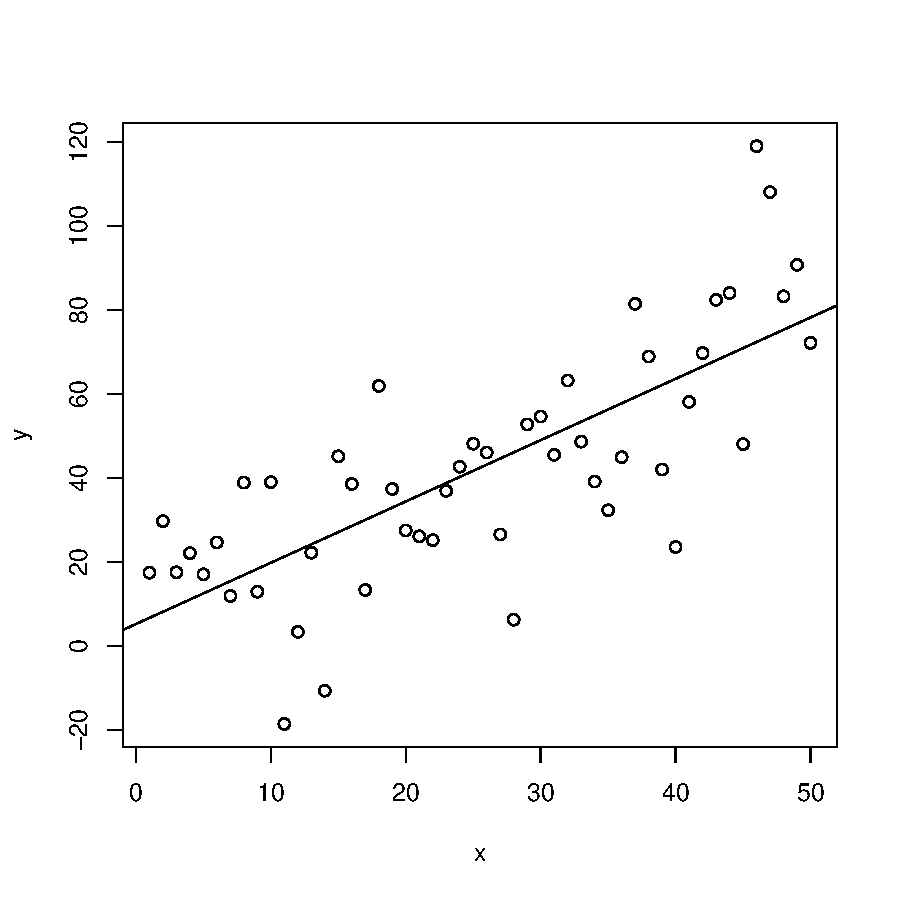
\includegraphics{sweaveTemplate-fig1}
\end{center}
\caption{Time series plot of MCMC output.}
\label{fig:fig1}
\end{figure}

Another way to look at the output is an autocorrelation plot.
Figure~\ref{fig:fig2} (page~\pageref{fig:fig2})
shows the time series plot made by the R statement
\begin{Schunk}
\begin{Sinput}
>     acf(out$batch)
\end{Sinput}
\end{Schunk}
\begin{figure}
\begin{center}
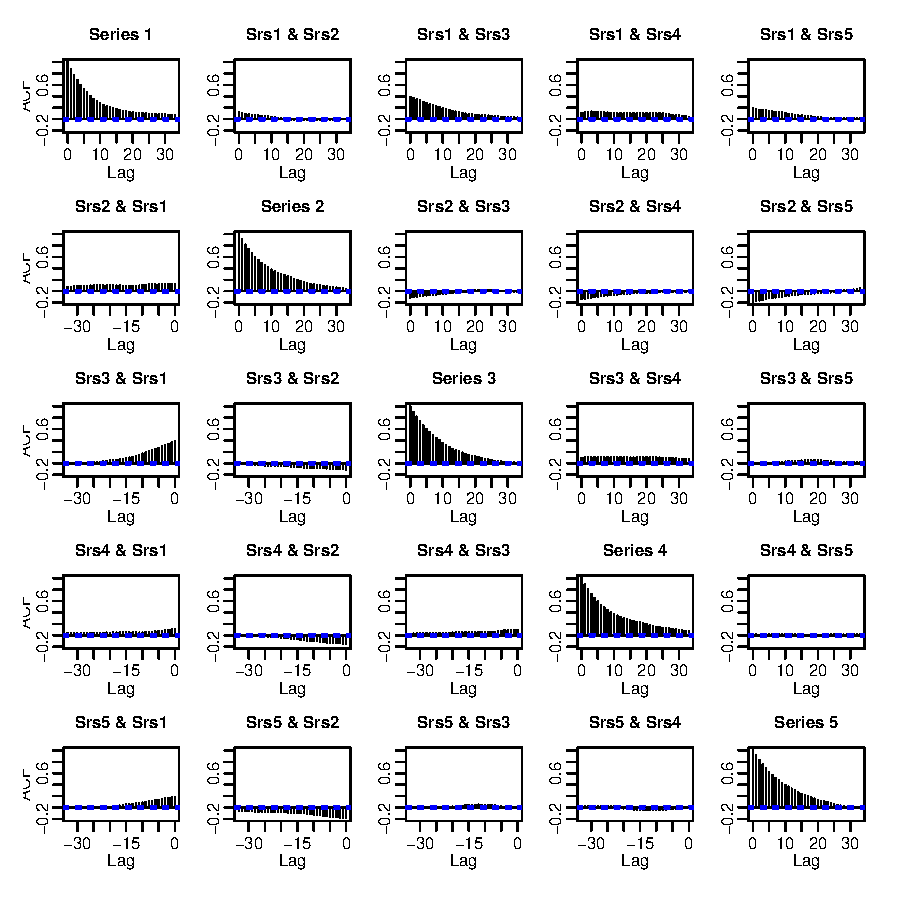
\includegraphics{sweaveTemplate-fig2}
\end{center}
\caption{Autocorrelation plot of MCMC output.}
\label{fig:fig2}
\end{figure}

As with any multiplot plot, these are a bit hard to read.  Readers are
invited to make the separate plots to get a better picture.
As with all ``diagnostic'' plots in MCMC, these don't ``diagnose''
subtle problems.  As
\begin{verbatim}
http://www.stat.umn.edu/~charlie/mcmc/diag.html
\end{verbatim}
says
\begin{quotation}
The purpose of regression diagnostics is to find obvious, gross,
embarrassing problems that jump out of simple plots.
\end{quotation}
The time series plots will show \emph{obvious} nonstationarity.
They will not show \emph{nonobvious} nonstationarity.  They
provide no guarantee whatsoever that your Markov chain is sampling
anything remotely resembling the correct stationary distribution
(with log unnormalized density \verb@lupost@).  In this very easy
problem, we do not expect any convergence difficulties and so believe
what the diagnostics seem to show, but one is a fool to trust such
diagnostics in difficult problems.

The autocorrelation plots seem to show that the
the autocorrelations are negligible after about lag 25.
This diagnostic inference is reliable if the sampler is actually
working (has nearly reached equilibrium) and worthless otherwise.
Thus batches of length 25 should be sufficient, but let's use
length 100 to be safe.

\section{Monte Carlo Estimates and Standard Errors}

\begin{Schunk}
\begin{Sinput}
>     out <- metrop(out, nbatch = 1e2, blen = 100,
+                   outfun = function(z, ...) c(z, z^2), x = x, y = y)
> out$accept
\end{Sinput}
\begin{Soutput}
[1] 0.2332
\end{Soutput}
\begin{Sinput}
> out$time
\end{Sinput}
\begin{Soutput}
   user  system elapsed 
  0.484   0.035   0.527 
\end{Soutput}
\end{Schunk}

We have added an argument \verb@outfun@ that gives the ``functional''
of the state we want to average.  For this problem we are interested
in both posterior mean and variance.  Mean is easy, just average the
variables in question.  But variance is a little tricky.  We need to
use the identity
$$
\var(X) = E(X^2) - E(X)^2
$$
to write variance as a function of two things that can be estimated
by simple averages.  Hence we want to average the state itself and
the squares of each component.  Hence our \verb@outfun@ returns
\verb@c(z, z^2)@ for an argument (the state vector) \verb@z@.

The \verb@...@ argument to \verb@outfun@ is required, since the
function is also passed the other arguments (here \verb@x@ and \verb@y@)
to \verb@metrop@.

\subsection{Simple Means}

The grand means (means of batch means) are
\begin{Schunk}
\begin{Sinput}
> apply(out$batch, 2, mean)
\end{Sinput}
\begin{Soutput}
 [1] 0.6531950 0.7920342 1.1701075 0.5077331 0.7488265
 [6] 0.5145751 0.7560775 1.4973807 0.3913837 0.7244162
\end{Soutput}
\end{Schunk}
The first 5 numbers are the Monte Carlo estimates of the posterior means.
The second 5 numbers are the Monte Carlo estimates of the posterior
absolute second moments.  We get the posterior variances by
\begin{Schunk}
\begin{Sinput}
> foo <- apply(out$batch, 2, mean)
> mu <- foo[1:5]
> sigmasq <- foo[6:10] - mu^2
> mu
\end{Sinput}
\begin{Soutput}
[1] 0.6531950 0.7920342 1.1701075 0.5077331 0.7488265
\end{Soutput}
\begin{Sinput}
> sigmasq
\end{Sinput}
\begin{Soutput}
[1] 0.08791134 0.12875924 0.12822924 0.13359081 0.16367507
\end{Soutput}
\end{Schunk}

Monte Carlo standard errors (MCSE) are calculated from the batch means.
This is simplest for the means.
\begin{Schunk}
\begin{Sinput}
> mu.mcse <- apply(out$batch[ , 1:5], 2, sd) / sqrt(out$nbatch)
> mu.mcse
\end{Sinput}
\begin{Soutput}
[1] 0.01224260 0.01417916 0.01793129 0.01468594 0.01582040
\end{Soutput}
\end{Schunk}
The extra factor \verb@sqrt(out$nbatch)@ arises because the batch means
have variance $\sigma^2 / b$ where $b$ is the batch length, which is
\verb@out$blen@,
whereas the overall means \verb@mu@ have variance $\sigma^2 / n$ where
$n$ is the total number of iterations, which is \verb@out$blen * out$nbatch@.

\subsection{Functions of Means}

To get the MCSE for the posterior variances we apply the delta method.
Let $u_i$ denote the sequence of batch means of the first kind for one
parameter and $\bar{u}$ the grand mean (the estimate of the posterior mean
of that parameter),
let $v_i$ denote the sequence of batch means of the second kind for the
same parameter and $\bar{v}$ the grand mean (the estimate of the posterior
second absolute moment of that parameter), and let $\mu = E(\bar{u})$ and
$\nu = E(\bar{v})$.  Then the delta method linearizes the nonlinear function
$$
g(\mu, \nu) = \nu - \mu^2
$$
as
$$
\Delta g(\mu, \nu) = \Delta \nu - 2 \mu \Delta \mu
$$
saying that
$$
g(\bar{u}, \bar{v}) - g(\mu, \nu)
$$
has the same asymptotic normal distribution as
$$
(\bar{v} - \nu) - 2 \mu (\bar{u} - \mu)
$$
which, of course, has variance \verb@1 / nbatch@ times that of
$$
(v_i - \nu) - 2 \mu (u_i - \mu)
$$
and this variance is estimated by
$$
\frac{1}{n_{\text{batch}}} \sum_{i = 1}^{n_{\text{batch}}}
\bigl[ (v_i - \bar{v}) - 2 \bar{u} (u_i - \bar{u}) \bigr]^2
$$
So
\begin{Schunk}
\begin{Sinput}
> u <- out$batch[ , 1:5]
> v <- out$batch[ , 6:10]
> ubar <- apply(u, 2, mean)
> vbar <- apply(v, 2, mean)
> deltau <- sweep(u, 2, ubar)
> deltav <- sweep(v, 2, vbar)
> foo <- sweep(deltau, 2, ubar, "*")
> sigmasq.mcse <- sqrt(apply((deltav - 2 * foo)^2, 2, mean) / out$nbatch)
> sigmasq.mcse
\end{Sinput}
\begin{Soutput}
[1] 0.004241637 0.007292224 0.007271390 0.007374833
[5] 0.008175832
\end{Soutput}
\end{Schunk}
does the MCSE for the posterior variance.

Let's just check that this complicated \verb@sweep@ and \verb@apply@ stuff
does do the right thing.
\begin{Schunk}
\begin{Sinput}
> sqrt(mean(((v[ , 2] - vbar[2]) - 2 * ubar[2] * (u[ , 2] - ubar[2]))^2) /
+     out$nbatch)
\end{Sinput}
\begin{Soutput}
[1] 0.007292224
\end{Soutput}
\end{Schunk}

\paragraph{Comment} Through version 0.5 of this vignette it contained
an incorrect procedure for calculating this MCSE, justified by a handwave.
Essentially, it said to use the standard deviation of the batch means called
\verb@v@ here, which appears to be very conservative.

\subsection{Functions of Functions of Means}

If we are also interested in the posterior standard deviation
(a natural question, although not asked on the exam problem),
the delta method gives its standard error in terms of that
for the variance
\begin{Schunk}
\begin{Sinput}
> sigma <- sqrt(sigmasq)
> sigma.mcse <- sigmasq.mcse / (2 * sigma)
> sigma
\end{Sinput}
\begin{Soutput}
[1] 0.2964985 0.3588304 0.3580911 0.3655008 0.4045678
\end{Soutput}
\begin{Sinput}
> sigma.mcse
\end{Sinput}
\begin{Soutput}
[1] 0.007152882 0.010161102 0.010152989 0.010088669
[5] 0.010104403
\end{Soutput}
\end{Schunk}

\section{A Final Run}

So that's it.  The only thing left to do is a little more precision
(the exam problem directed ``use a long enough run of your Markov chain
sampler so that the MCSE are less than 0.01'')
\begin{Schunk}
\begin{Sinput}
> out <- metrop(out, nbatch = 5e2, blen = 400, x = x, y = y)
> out$accept
\end{Sinput}
\begin{Soutput}
[1] 0.235155
\end{Soutput}
\begin{Sinput}
> out$time
\end{Sinput}
\begin{Soutput}
   user  system elapsed 
  9.689   0.635  10.350 
\end{Soutput}
\begin{Sinput}
> foo <- apply(out$batch, 2, mean)
> mu <- foo[1:5]
> sigmasq <- foo[6:10] - mu^2
> mu
\end{Sinput}
\begin{Soutput}
[1] 0.6624650 0.7941013 1.1712710 0.5066326 0.7261414
\end{Soutput}
\begin{Sinput}
> sigmasq
\end{Sinput}
\begin{Soutput}
[1] 0.09189246 0.13323054 0.13230811 0.12871293 0.15978638
\end{Soutput}
\begin{Sinput}
> mu.mcse <- apply(out$batch[ , 1:5], 2, sd) / sqrt(out$nbatch)
> mu.mcse
\end{Sinput}
\begin{Soutput}
[1] 0.002960128 0.003647420 0.003787855 0.003632080
[5] 0.004273624
\end{Soutput}
\begin{Sinput}
> u <- out$batch[ , 1:5]
> v <- out$batch[ , 6:10]
> ubar <- apply(u, 2, mean)
> vbar <- apply(v, 2, mean)
> deltau <- sweep(u, 2, ubar)
> deltav <- sweep(v, 2, vbar)
> foo <- sweep(deltau, 2, ubar, "*")
> sigmasq.mcse <- sqrt(apply((deltav - 2 * foo)^2, 2, mean) / out$nbatch)
> sigmasq.mcse
\end{Sinput}
\begin{Soutput}
[1] 0.001044801 0.001725900 0.001518322 0.001553468
[5] 0.002010717
\end{Soutput}
\begin{Sinput}
> sigma <- sqrt(sigmasq)
> sigma.mcse <- sigmasq.mcse / (2 * sigma)
> sigma
\end{Sinput}
\begin{Soutput}
[1] 0.3031377 0.3650076 0.3637418 0.3587658 0.3997329
\end{Soutput}
\begin{Sinput}
> sigma.mcse
\end{Sinput}
\begin{Soutput}
[1] 0.001723311 0.002364198 0.002087087 0.002165017
[5] 0.002515076
\end{Soutput}
\end{Schunk}
and some nicer output, which is presented in three tables
constructed from the R variables defined above
using the R \verb@xtable@ command in the \verb@xtable@ library.

First the posterior means,
\begin{table}[ht]
\caption{Posterior Means}
\label{tab:mu}
\begin{center}
% latex table generated in R 2.14.0 by xtable 1.6-0 package
% Sun Jan 15 18:01:04 2012
\begin{tabular}{lccccc}
  \hline
 & constant & $x_1$ & $x_2$ & $x_3$ & $x_4$ \\ 
  \hline
estimate & 0.6625 & 0.7941 & 1.1713 & 0.5066 & 0.7261 \\ 
  MCSE & 0.0030 & 0.0036 & 0.0038 & 0.0036 & 0.0043 \\ 
   \hline
\end{tabular}\end{center}
\end{table}
then the posterior variances (table on page~\pageref{tab:sigmasq}),
\begin{table}[ht]
\caption{Posterior Variances}
\label{tab:sigmasq}
\begin{center}
% latex table generated in R 2.14.0 by xtable 1.6-0 package
% Sun Jan 15 18:01:04 2012
\begin{tabular}{lccccc}
  \hline
 & constant & $x_1$ & $x_2$ & $x_3$ & $x_4$ \\ 
  \hline
estimate & 0.0919 & 0.1332 & 0.1323 & 0.1287 & 0.1598 \\ 
  MCSE & 0.0010 & 0.0017 & 0.0015 & 0.0016 & 0.0020 \\ 
   \hline
\end{tabular}\end{center}
\end{table}
and finally the posterior standard deviations
(table on page~\pageref{tab:sigma}).
\begin{table}[ht]
\caption{Posterior Standard Deviations}
\label{tab:sigma}
\begin{center}
% latex table generated in R 2.14.0 by xtable 1.6-0 package
% Sun Jan 15 18:01:04 2012
\begin{tabular}{lccccc}
  \hline
 & constant & $x_1$ & $x_2$ & $x_3$ & $x_4$ \\ 
  \hline
estimate & 0.3031 & 0.3650 & 0.3637 & 0.3588 & 0.3997 \\ 
  MCSE & 0.0017 & 0.0024 & 0.0021 & 0.0022 & 0.0025 \\ 
   \hline
\end{tabular}\end{center}
\end{table}

Note for the record that the all the results presented in the tables
are from ``one long run'' where long here took only
9.689 seconds (on whatever computer it was run on).

\section{New Variance Estimation Functions}

A new function \texttt{initseq} estimates variances in the Markov chain
central limit theorem (CLT) following the methodology introduced by
\citet[Section~3.3]{practical}.  These methods only apply to scalar-valued
functionals of
reversible Markov chains, but the Markov chains produced by the \texttt{metrop}
function satisfy this condition, even, as we shall see below, when batching
is used.

Rather than redo the Markov chains in the preceding material, we just look
at a toy problem, an AR(1) time series, which can be simulated in one line
of R.  This is the example on the help page for \texttt{initseq}.
\begin{Schunk}
\begin{Sinput}
> n <- 2e4
> rho <- 0.99
> x <- arima.sim(model = list(ar = rho), n = n)
\end{Sinput}
\end{Schunk}
The time series \texttt{x} is a reversible Markov chain and trivially
a scalar-valued functional of a Markov chain.

Define
\begin{equation} \label{eq:little}
\gamma_k = \cov(X_i, X_{i + k})
\end{equation}
where the covariances refer to the stationary Markov chain having the
same transition probabilities as \texttt{x}.  Then the variance in the CLT
is
$$
\sigma^2 = \gamma_0 + 2 \sum_{k = 1}^\infty \gamma_k
$$
\citep[Theorem~2.1]{practical}, that is,
$$
\bar{x}_n \approx \text{Normal}\left(\mu, \frac{\sigma^2}{n}\right),
$$
where $\mu = E(X_i)$ is the quantity being estimated by MCMC (in this
toy problem we know $\mu = 0$).

Naive estimates of $\sigma^2$ obtained by plugging in empirical
estimates of the gammas do not provide consistent estimation
\citep[Section~3.1]{practical}.  Thus the scheme implemented
by the R function \texttt{initseq}.  Define
\begin{equation} \label{eq:big}
\Gamma_k = \gamma_{2 k} + \gamma_{2 k + 1}
\end{equation}
\citet[Theorem~3.1]{practical} says that $\Gamma_k$ considered as a function
of $k$ is strictly positive, strictly decreasing, and strictly convex
(provided we are, as stated above, working with a reversible Markov chain).
Thus it makes sense to use estimators that use these properties.
The estimators implemented by the R function \texttt{initseq} and
described by \citet[Section~3.3]{practical} are conservative-consistent
in the sense of Theorem~3.2 of that section.

Figure~\ref{fig:gamma} (page~\pageref{fig:gamma})
shows the time series plot made by the R statement
\begin{Schunk}
\begin{Sinput}
> out <- initseq(x)
> plot(seq(along = out$Gamma.pos) - 1, out$Gamma.pos,
+      xlab = "k", ylab = expression(Gamma[k]), type = "l")
> lines(seq(along = out$Gamma.dec) - 1, out$Gamma.dec, lty = "dotted")
> lines(seq(along = out$Gamma.con) - 1, out$Gamma.con, lty = "dashed")
\end{Sinput}
\end{Schunk}
\begin{figure}
\begin{center}
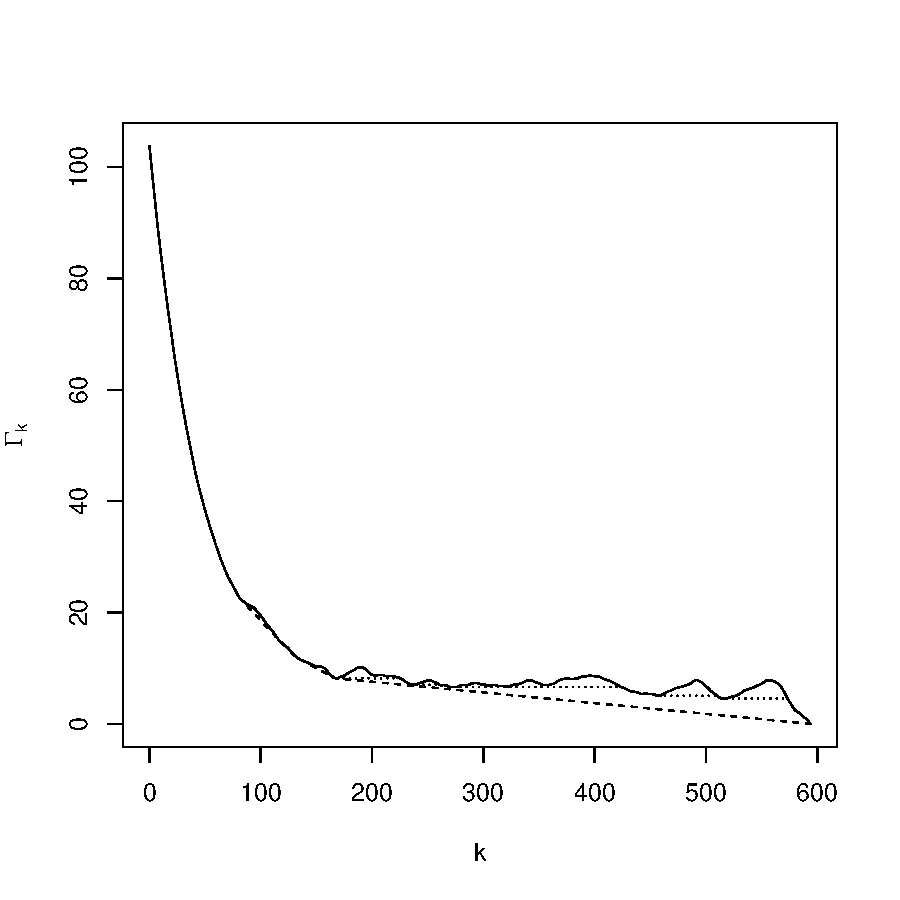
\includegraphics{sweaveTemplate-figgam}
\end{center}
\caption{Plot ``Big Gamma'' defined by \eqref{eq:little} and \eqref{eq:big}.
         Solid line, initial positive sequence estimator.
         Dotted line, initial monotone sequence estimator.
         Dashed line, initial convex sequence estimator.}
\label{fig:gamma}
\end{figure}
One can use whichever curve one chooses, but there is no reason, now that
the \texttt{initseq} function makes the computation trivial, to use the
initial convex sequence.

Of course, one is not interested in Figure~\ref{fig:gamma}, except
perhaps when explaining the methodology.  What is actually important
is the estimate of $\sigma^2$, which is given by
\begin{Schunk}
\begin{Sinput}
>     out$var.con
\end{Sinput}
\begin{Soutput}
[1] 14386.32
\end{Soutput}
\begin{Sinput}
> (1 + rho) / (1 - rho) * 1 / (1 - rho^2)
\end{Sinput}
\begin{Soutput}
[1] 10000
\end{Soutput}
\end{Schunk}
where for comparison we have given the exact theoretical value of $\sigma^2$,
which, of course, is never available in a non-toy problem.

These initial sequence estimators seem, at first sight to be a competitor
for the method of batch means.  However, appearances can be deceiving.
The two methods are complementary.  The sequence of batch means is itself
a scalar-valued functional of a reversible Markov chain.  Hence the
initial sequence estimators can be applied to it.
\begin{Schunk}
\begin{Sinput}
> blen <- 5
> x.batch <- apply(matrix(x, nrow = blen), 2, mean)
> bout <- initseq(x.batch)
\end{Sinput}
\end{Schunk}
Because the batch length is too short, the variance of the batch means
does not estimate $\sigma^2$.  We must account for the autocorrelation
of the batches, shown in Figure~\ref{fig:gambat}.
\begin{Schunk}
\begin{Sinput}
> plot(seq(along = bout$Gamma.con) - 1, bout$Gamma.con,
+      xlab = "k", ylab = expression(Gamma[k]), type = "l")
\end{Sinput}
\end{Schunk}
\begin{figure}
\begin{center}
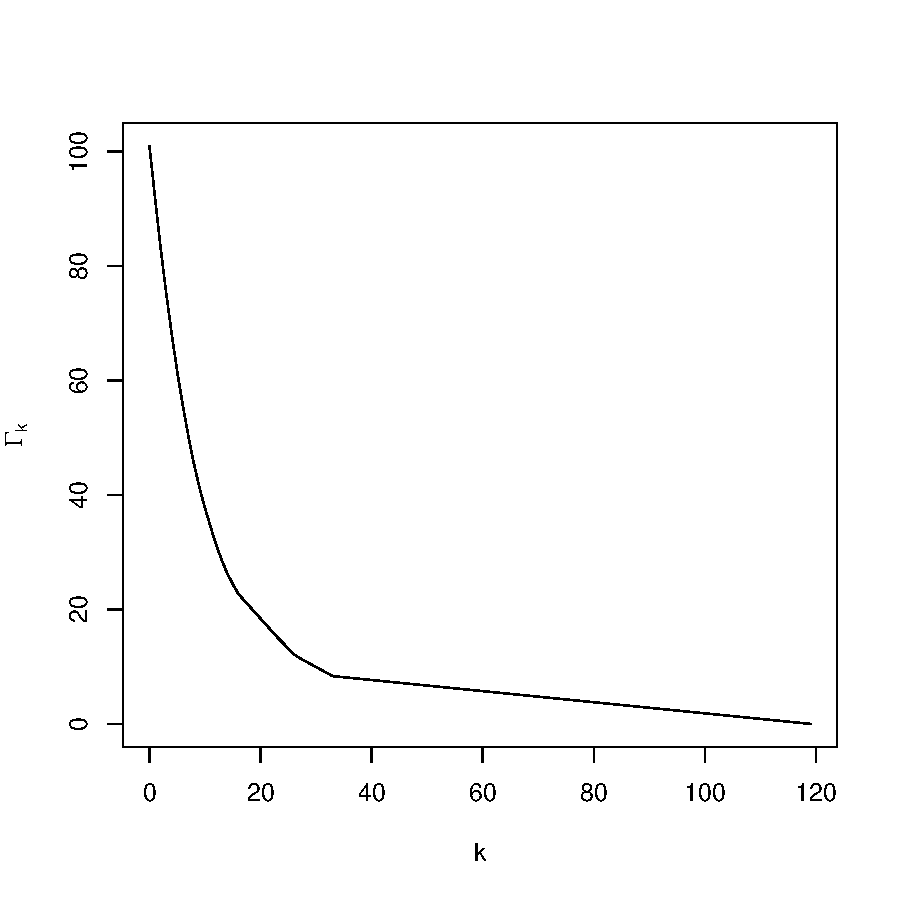
\includegraphics{sweaveTemplate-figgambat}
\end{center}
\caption{Plot ``Big Gamma'' defined by \eqref{eq:little} and \eqref{eq:big}
         for the sequence of batch means (batch length 5).
         Only initial convex sequence estimator is shown.}
\label{fig:gambat}
\end{figure}
Because the the variance is proportional to one over the batch length,
we need to multiply by the batch length to estimate the $\sigma^2$
    for the original series.
\begin{Schunk}
\begin{Sinput}
>     out$var.con
\end{Sinput}
\begin{Soutput}
[1] 14386.32
\end{Soutput}
\begin{Sinput}
> bout$var.con * blen
\end{Sinput}
\begin{Soutput}
[1] 14466.75
\end{Soutput}
\end{Schunk}
Another way to look at this is that the MCMC estimator of $\mu$ is
either \texttt{mean(x)} or \texttt{mean(x.batch)}.  And the variance
must be divided by the sample size to give standard errors.  So either
\begin{Schunk}
\begin{Sinput}
> mean(x) + c(-1, 1) * qnorm(0.975) * sqrt(out$var.con / length(x))
\end{Sinput}
\begin{Soutput}
[1] -0.5078635  2.8167249
\end{Soutput}
\begin{Sinput}
> mean(x.batch) + c(-1, 1) * qnorm(0.975) * sqrt(bout$var.con / length(x.batch))
\end{Sinput}
\begin{Soutput}
[1] -0.5125039  2.8213653
\end{Soutput}
\end{Schunk}
is an asymptotic 95\% confidence interval for $\mu$.  Just divide by
the relevant sample size.

\begin{thebibliography}{}

\bibitem[Gelman et al.(1996)Gelman, Roberts, and Gilks]{grg}
Gelman, A., G.~O. Roberts, and W.~R. Gilks (1996).
\newblock Efficient Metropolis jumping rules.
\newblock In \emph{Bayesian Statistics, 5 (Alicante, 1994)}, pp.~599--607.
Oxford University Press.

\bibitem[Geyer(1992)]{practical}
Geyer, C.~J. (1992).
\newblock Practical Markov chain Monte Carlo (with discussion).
\newblock \emph{Statistical Science}, 7, 473--511.

\bibitem[Geyer and Thompson(1995)]{geyer-temp}
Geyer, C.~J. and E.~A. Thompson (1995).
\newblock Annealing Markov chain Monte Carlo with applications to
ancestral inference.
\newblock \emph{Journal of the American Statistical Association}, 90, 909--920.

\end{thebibliography}

\end{document}
